%
% Use the standard article template.
%
\documentclass{article}

% The geometry package allows for easy page formatting.
\usepackage{geometry}
\geometry{letterpaper}

% Load up special logo commands.
\usepackage{doc}

% Package for formatting URLs.
\usepackage{url}

% Packages and definitions for graphics files.
\usepackage{graphicx}
\usepackage{epstopdf}
\DeclareGraphicsRule{.tif}{png}{.png}{`convert #1 `dirname #1`/`basename #1 .tif`.png}

%
% Set the title, author, and date.
%

\begin{document}

\title{Accelerometer data classification using Neural Networks}
\author{ Sameer, Shantanu, Rekah, Eera}

% Add various lists on new pages.
\tableofcontents
\pagebreak
\listoffigures

% Start the paper on a new page.
\pagebreak


% Add the title section.
\maketitle

% Add an abstract.
\abstract{
Human activity is a great source for building new kind of services that take the current status of the user into consideration.
Equipping a service provided by a phone application with the context of the user results in richer and more engaging services. In 
this work we present a neural based classifier that is able to detect the status of the human body from readings of 
accelerometers placed on different parts of the body. We show how different configuration of the neural network and 
data preprocessing can change the accuracy of our prediction, we also show how we can predict the movement using one 
accelerometer reading to simulate the effect of having a mobile device in users pocket or a smart watch attached to 
the user's wrist. To the best of our knowledge this is the first study that considers a single source of data and 
achieves (96\%) accuracy. 
}

\section{Introduction}
\label{introduction}

With the increasing use of smart mobile devices new opportunities are present for richer and more engaging services 
that cater to every need of its users. Most of these smart devices are equipped with accelerometers that give an
indication of of the relative position of the device and its user at any point in time. Using this data to identify the 
status of body movement provides an accurate record of the physical activity of the user which has applications related 
to the health care and interactive design for mobile devices' applications. 

In this work we seek to build a neural network based classifier that is able to correctly identify a pattern of human body 
movement from a series of readings, we discuss different design choices and report their impact on prediction accuracy. The 
rest of this report goes as follows; section~\ref{DataSet} describes the dataset we are using, section~\ref{methodology} describes 
the methodology we used, section~\ref{conclusion} discusses a summary of the results we are getting and includes ideas for future work.


\section{Data Set}
\label{DataSet}

Raw data we are using are based on the work by~\cite{ugulino2012wearable}. The data set report 8 hours of activity of 4 subject tests 
of varying age , weight, height and gender. Each subject provided two hours of activity of postures varying between (Standing,
sitting down, sitting , standing up and walking). The data provided is a continuous stream of reading from sensors placed of four 
parts of the body, waist, arm, leg and foot. Figure~\ref{acc_placement} shows the places of these accelerators~\cite{ugulino2012wearable}.
Figure~\ref{sample_dist} shows the distribution of the postures among the samples.

Along with the three dimensional input from each accelerometer,which is adds up to twelve readings for each time step, the data set 
also provides some biometrics that are subject specific. This could help improving the prediction accuracy given that different users might
move differently and having these metrics helps the neural network account for that. These biometrics include the following: 

\begin{enumerate}
  \item Age: Humans movement pattern tend to change\\evolve in different ages. 
  \item Weight: Weight affects the way humans move which also affects the accelerometer data.
  \item Height: Reading along the Y-direction (height direction) are affected by subject's height.
  \item Gender: Males and females have different patterns for movement, especially for walking. 
\end{enumerate}  


\begin{figure}
\centering
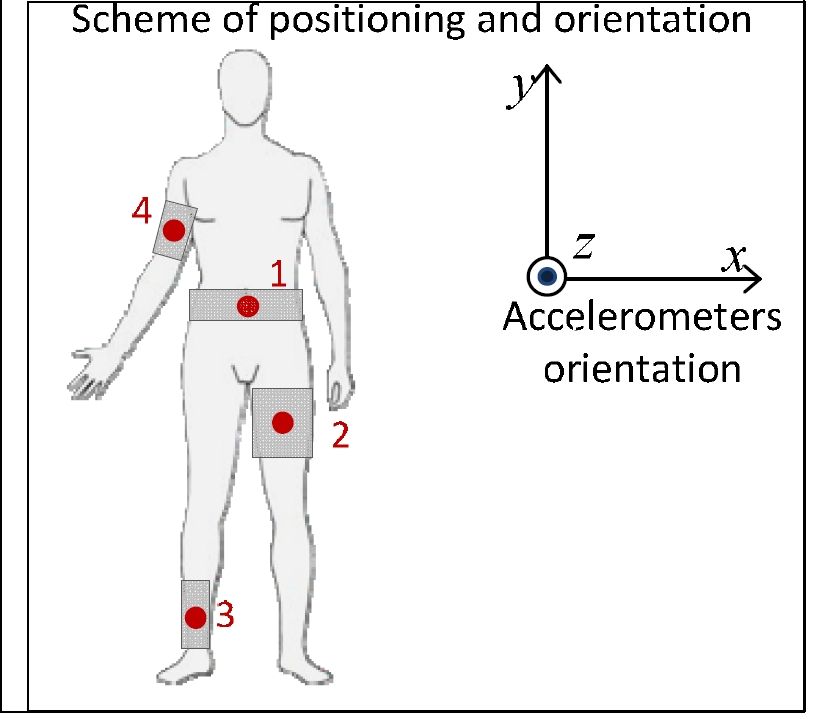
\includegraphics[width=2.5in]{acc_placement}
\caption{Accelerometer Placement}
\label{acc_placement}
\end{figure}

\begin{figure}
\centering
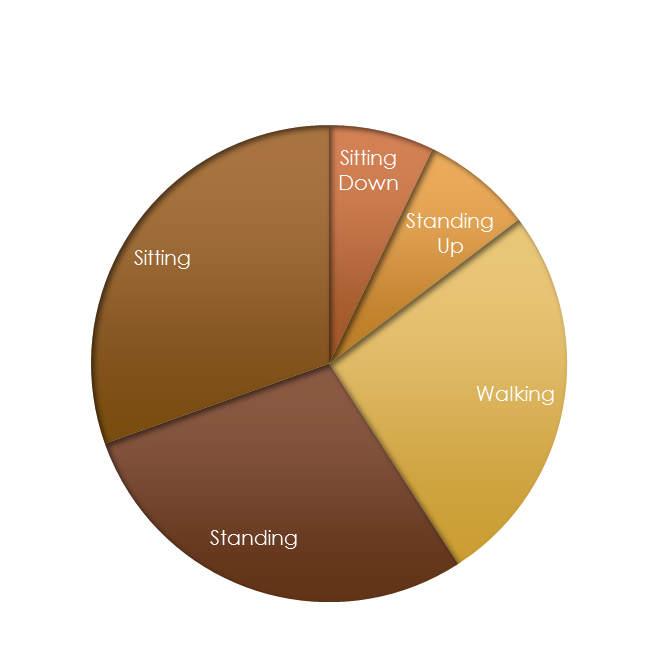
\includegraphics[width=3.0in]{samples_piechart}
\caption{Sample data distribution}
\label{sample_dist}
\end{figure}

\section{Frameworks}
\label{tools}

During the course of our experiments we tried different tools and libraries before settling on doing all of out experiments using 
Matlab~\cite{MATLAB:2014}. We used used the following tools:

\subsection{PyBrain}
PyBrain~\cite{pybrain2010jmlr} is a strong and modular Python library for building machine learning applications. It
support for building reinforcement learning and Neural network based learning. It allows for building flexible architecture for different
kind of networks (Feed Forward, Recurrent) it also has predefined layers for different layer for  network architectures like 
LSTM~\cite{hochreiter1997long} and Linear layers. It also allows for different kinds of activation functions. We used PyBrain to train FFN 
on raw entries of the data with  different number of layers and number of neurons in hidden layers, the maximum classification 
accuracy we got was 73\% after around 200 epoch steps, feeding the network seven consecutive rows at a time  raised the accuracy to 80\%.
We stopped experimenting with PyBrain because of the high execution time we were facing. Training a thousand steps for the FFN with 
seven row input took about 5 hours, we had to look for some other platform. 


\subsection{NeuroLab}
NeuroLab~\cite{NeuroLab:Online} is a simple and powerful SciPy Python Python based library for building Neural Network. It is not as 
configurable or developed as PyBrain. Unfortunately, given the large data set we had and due the fact that this is a Pure Python 
based library we faced the same problems of high execution time. 

\subsection{Other libraries}
These include Bain.js~\cite{BrainJs} and Cuda-Convert~\cite{Cuda-convert}. Initial use of these two libraries didn't provide any promising
results they showed to be not up to the speed we needed  as well.  


\section{Methodology}
\DeclareGraphicsExtensions{.pdf,.png,.jpeg}
\label{methodology}

Previous work in detecting the body posture~\cite{ugulino2012wearable} used decision tree algorithms, namely C4.5, with intensive 
data preprocessing and feature extraction before actually using the data for classification; work include finding the roll and 
pitch angles for the body and also the variance in roll and pitch. In this work we opted for doing as possible of data preprocessing
and to let the neural network the feature extraction. We try to train our network with the following variants:

\begin{enumerate}
  \item Using unprocessed rows and feeding them to the network, section~\ref{simple_rows} discusses that.
  \item Using deltas of two consecutive rows or more than two rows, section~\ref{consecutive_rows} discusses that. 
  \item A person specific learner where we only do the training for one person for increased accuracy. 
  \item Use only one accelerometer to detect body posture. This gives a more realistic use case where the user only 
        has one source of data; a smart phone. Section~\ref{single_acc} discusses that.
\end{enumerate}  

Doing these operations and trying different versions we managed to achieve up to 99.85\% classification accuracy which is higher 
than the one achieved by~\cite{ugulino2012wearable} which accounted to 99.4\%. 


\subsection{Classification using raw rows}
\label{simple_rows}
For an initial start we built Neural networks that take all the readings in separate rows. We relied on the idea that even though the
human goes through the same stages between standing up and sitting down the subject might actually have a subtle difference in the exact
points that the accelerometer reads the data at TODO SHANTANU I NEED YOUR RUN FOR THIS !!!

\subsection{A Moving window}
\label{consecutive_rows}
As described in section~\ref{DataSet} the rows of data we have are actually consecutive in time, mashing more than one row into single input
to the Neural Network gives a sense of of this movement for the network to learn; for this we came up with the idea of a moving window.
To build this moving window we take 8 consecutive row, accounting for 1 second of time, and we find the difference in readings between the 
beginning and the end of the window. We tried different network configuration and architectures, increasing the number of Neurons gave some
good results with best prediction accuracy for validation data of 99.7\%. Figure~\ref{14_confusion} shows the confusion matrix and 
accuracy for a network of 372 neurons in the hidden layer shown in in figure~\ref{14_net}, figure~\ref{14_train} shows the gradient values 
along the training steps and the number of validation checks.
\begin{figure}
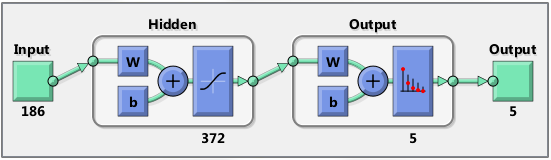
\includegraphics{14_net}
\caption{Neural Network for moving window}
\label{14_net}
\end{figure}

\begin{figure}
\centering
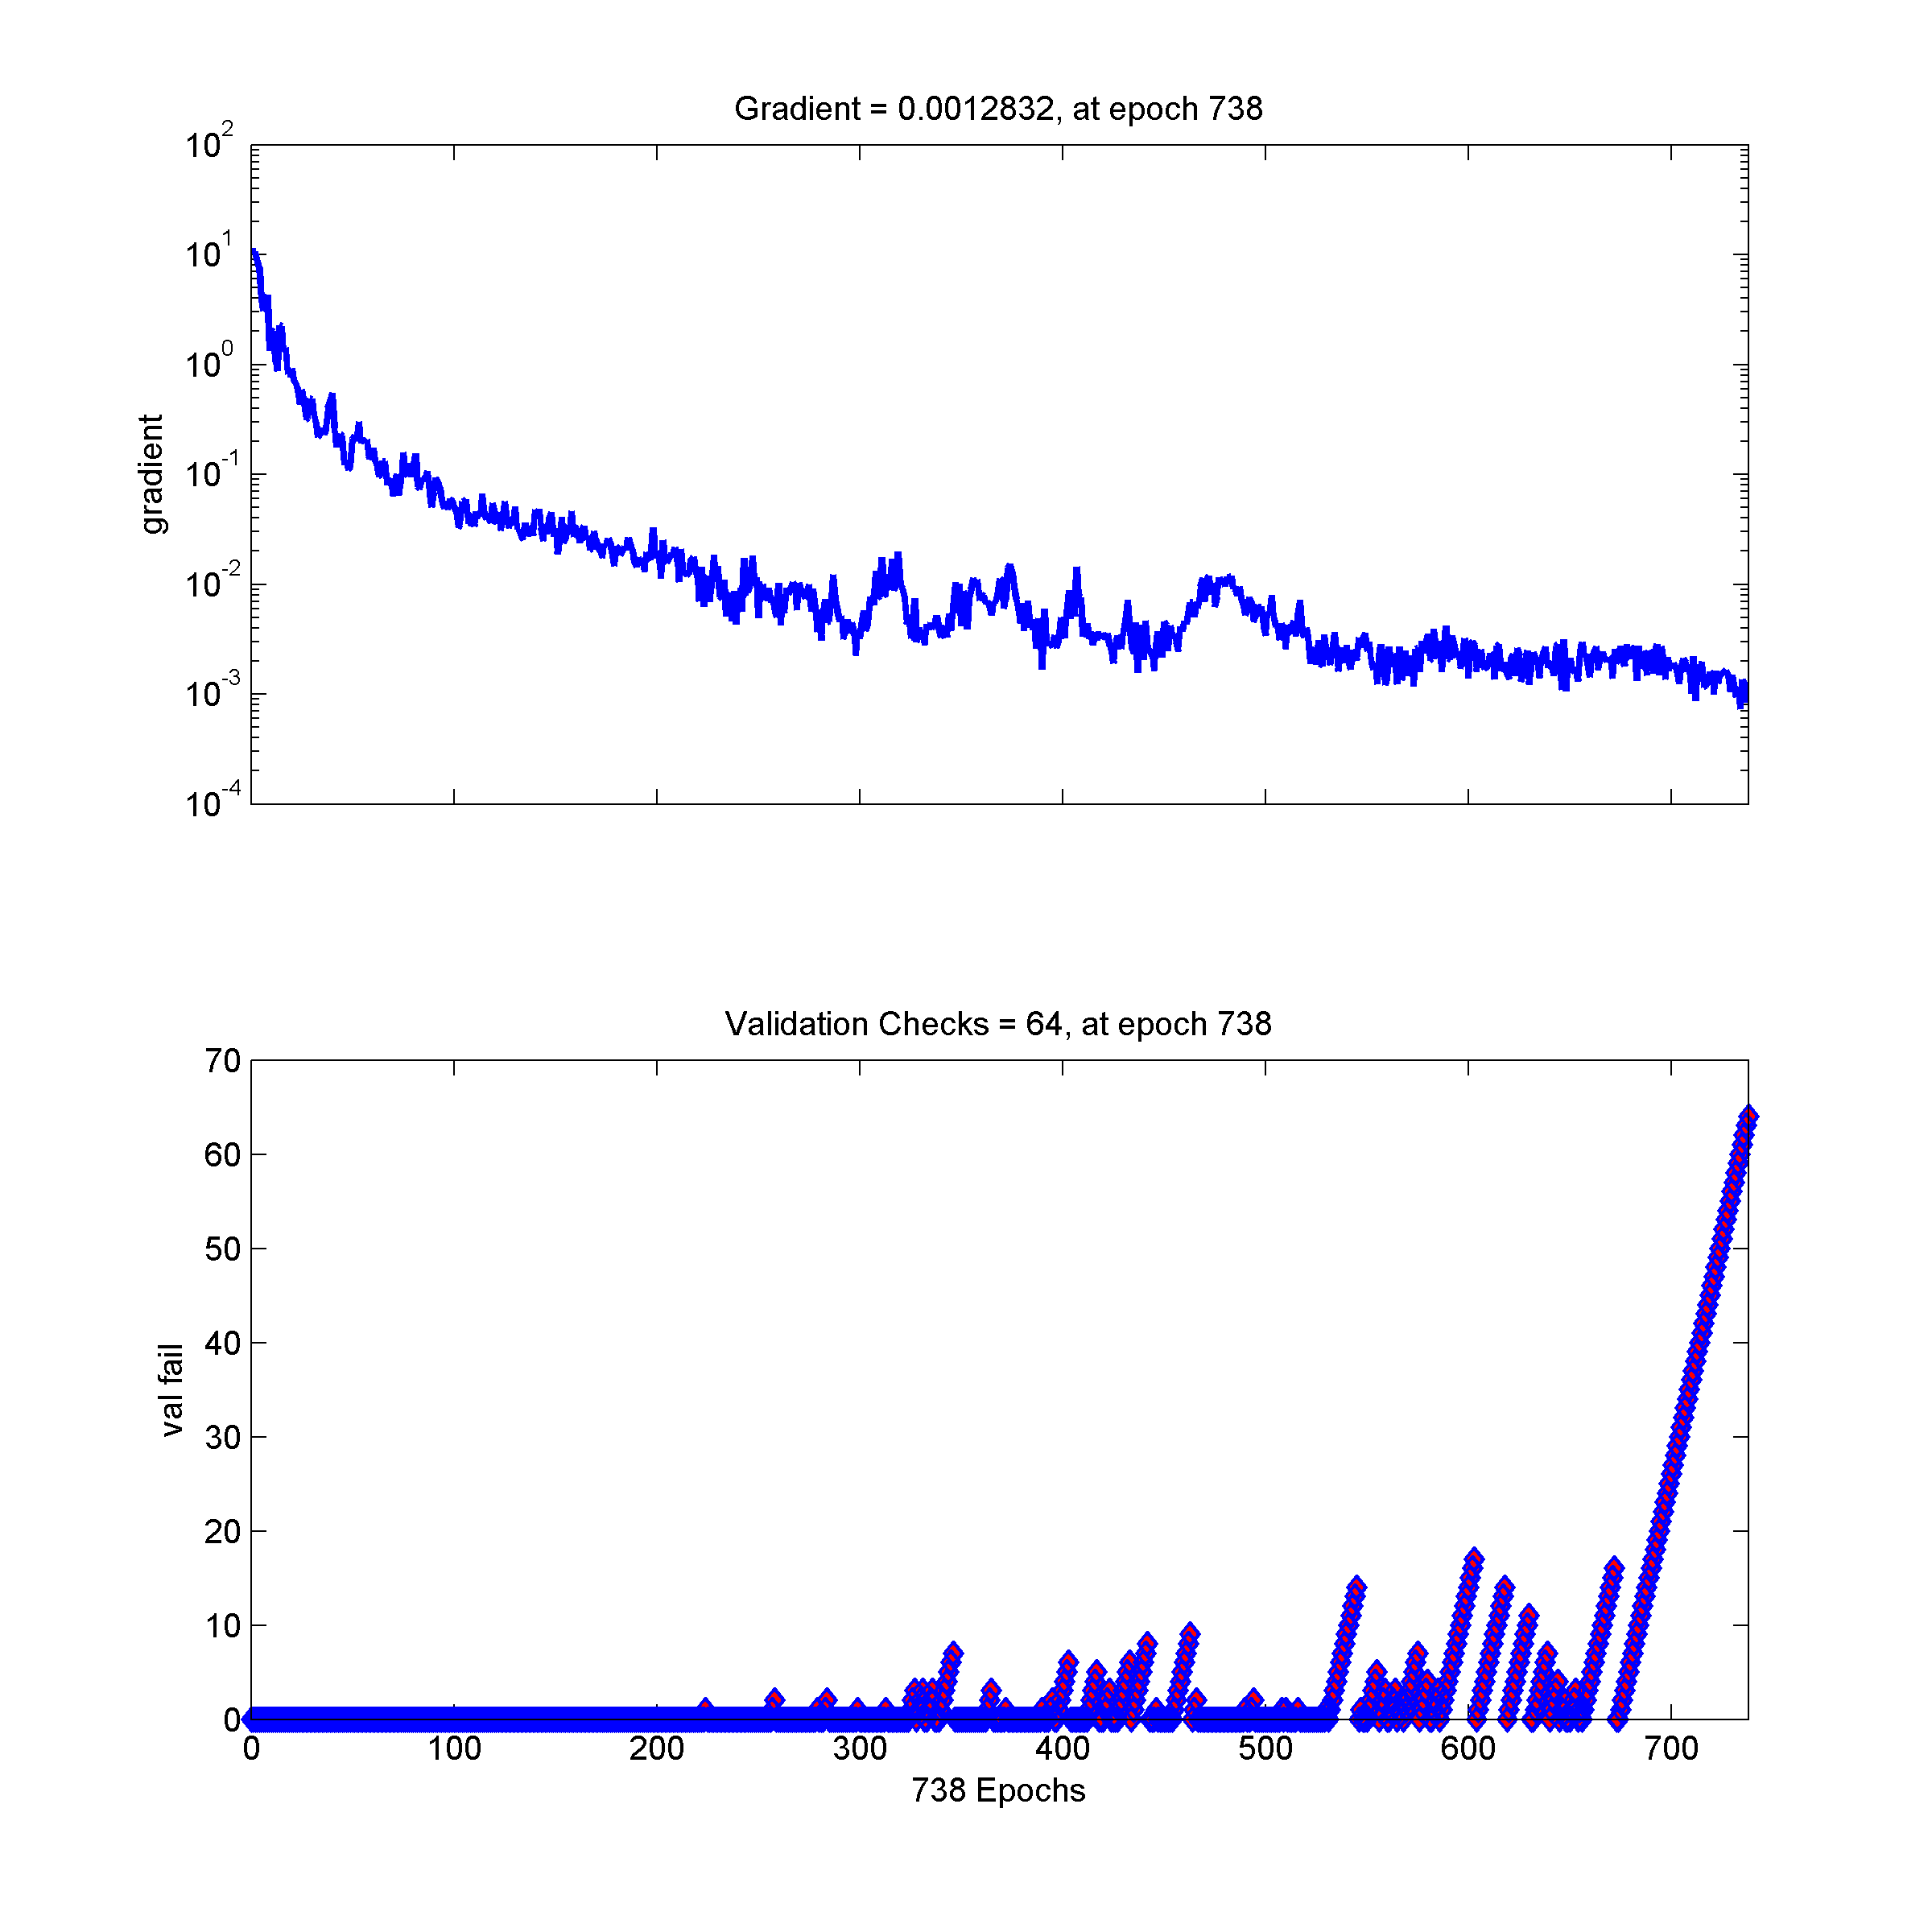
\includegraphics[width=3in]{14_train}
\caption{Gradient values and validation checks}
\label{14_train}
\end{figure}

\begin{figure}
\centering
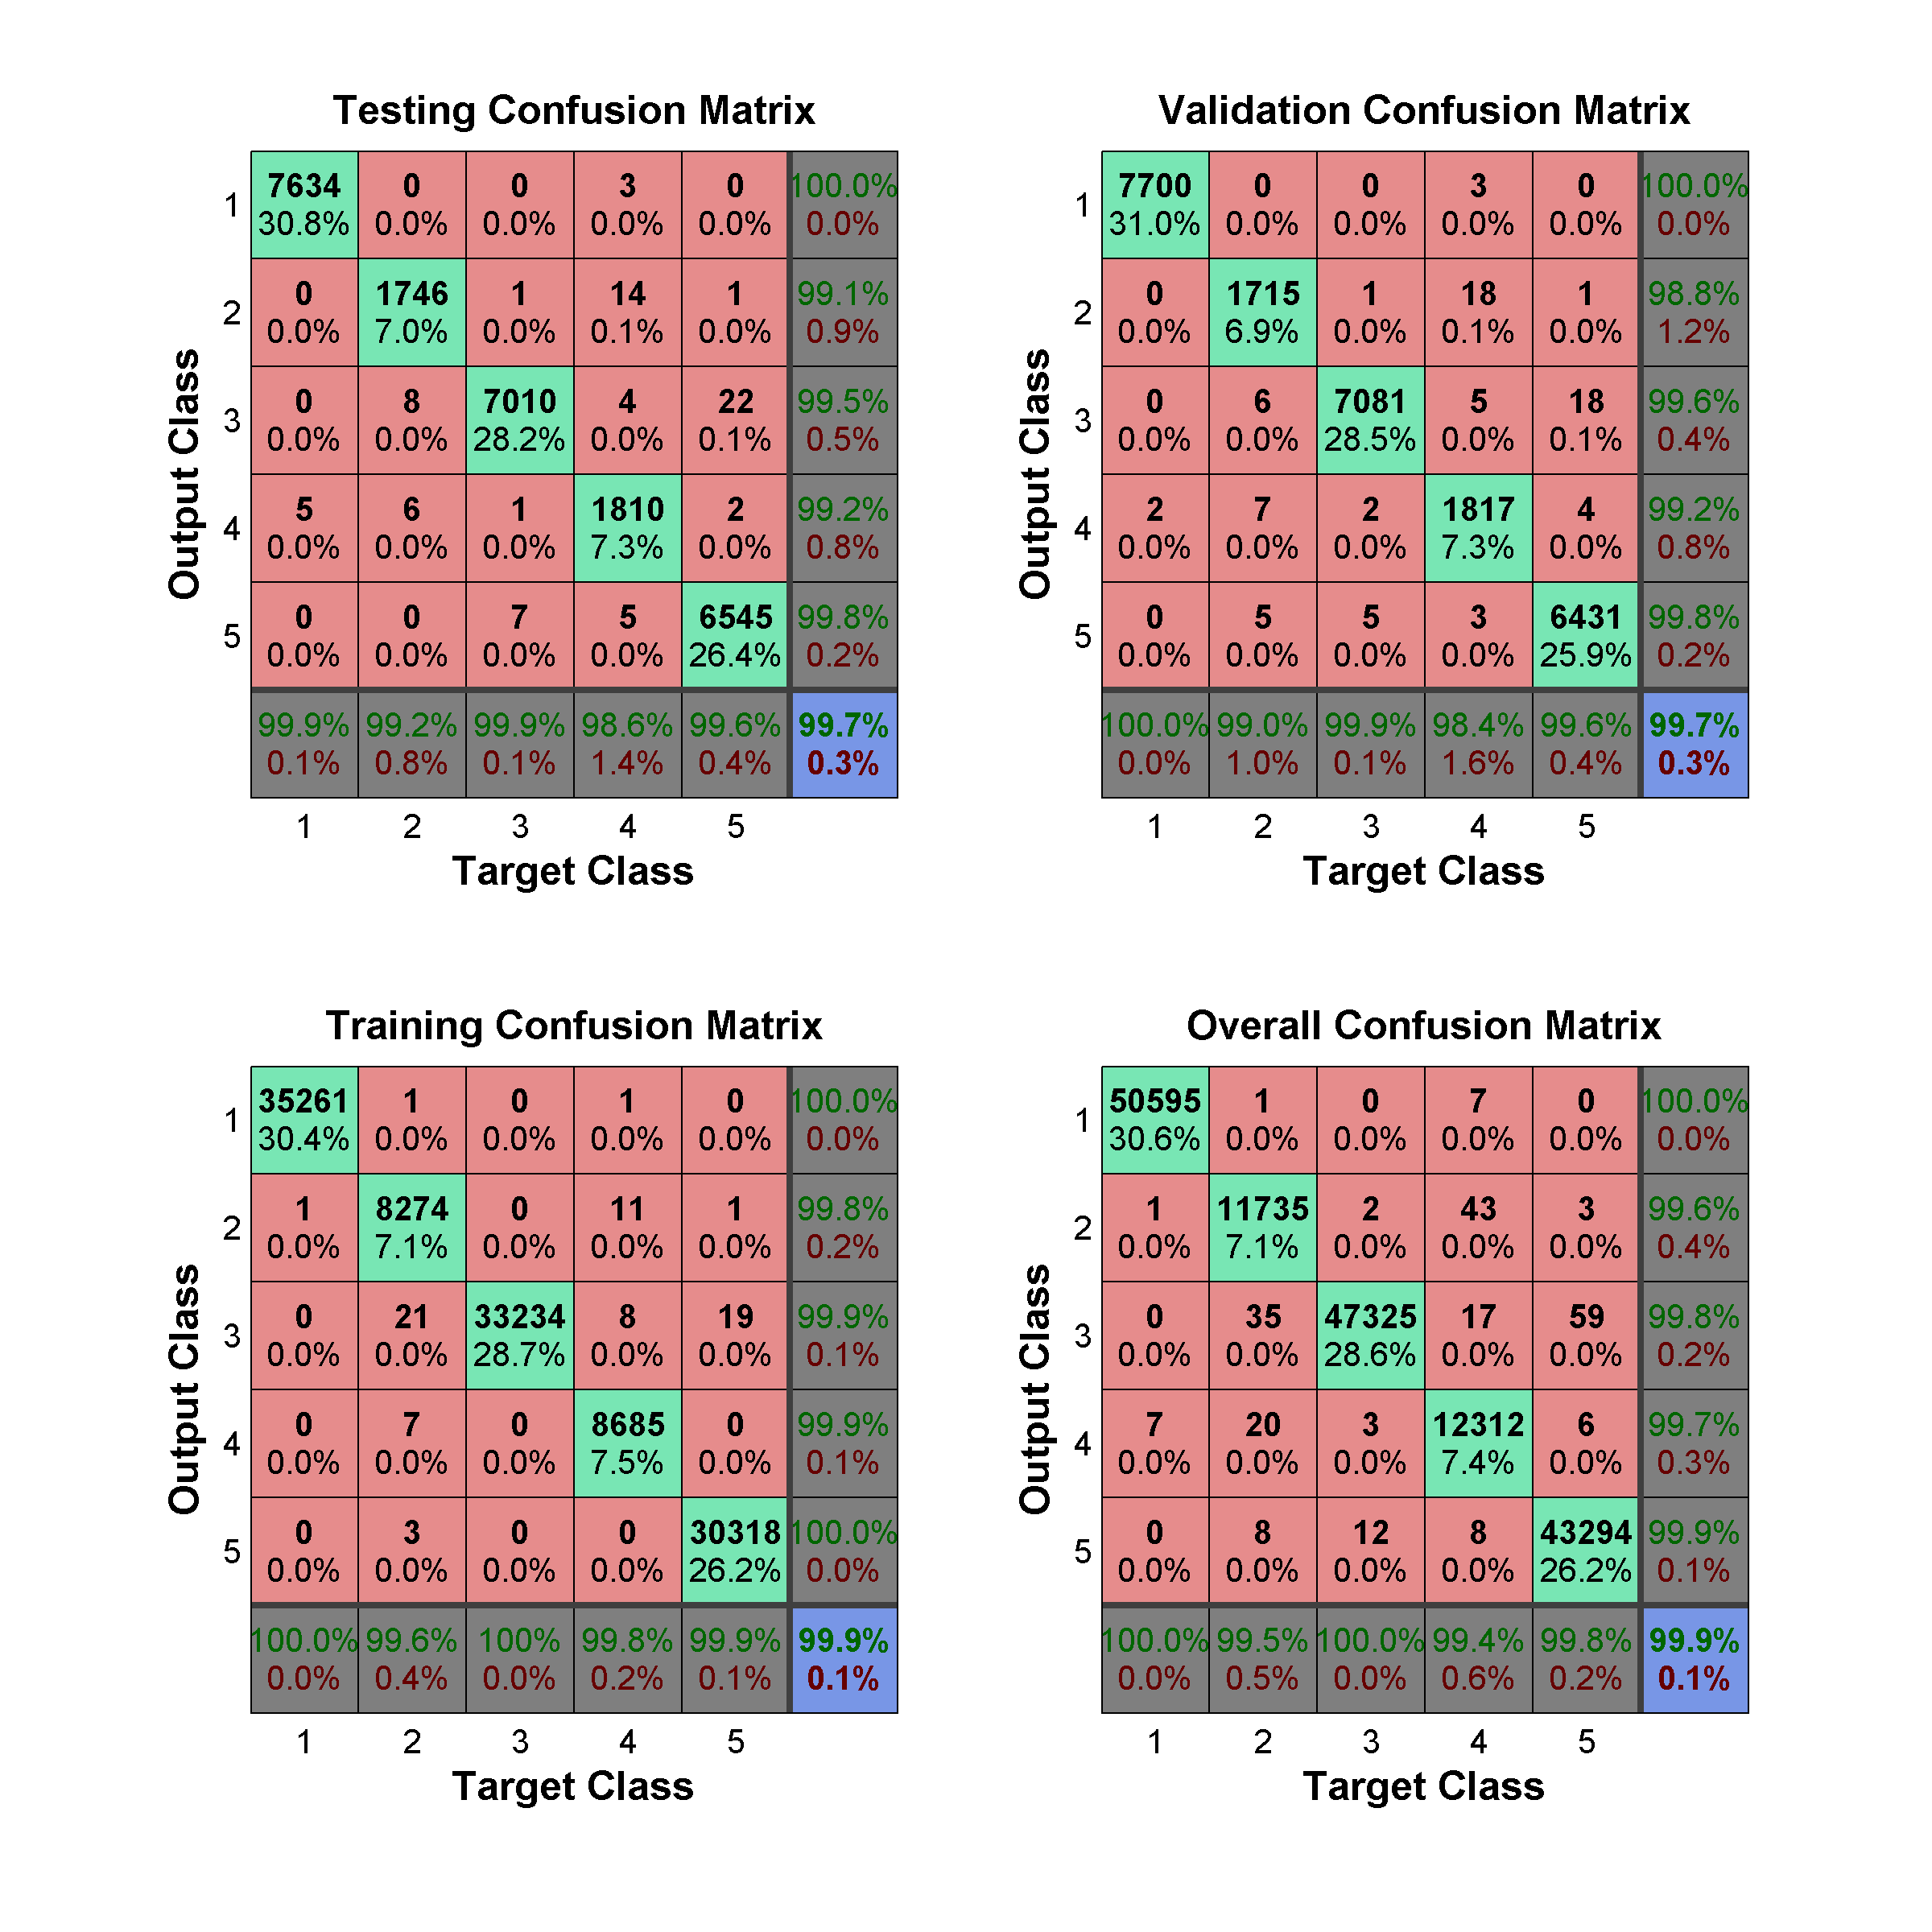
\includegraphics[width=3in]{14_confusion}
\caption{Confusion matrix results for moving window}
\label{14_confusion}
\end{figure}


\subsection{Single source of data} 
\label{single_acc}
Good prediction accuracy we achieved with readings from four different accelerometers made us think of what accuracy we can sustain with 
only one accelerometer. In part this also mimics the situation we have in real life where the subject holds a phone in his hand or in her
pocket. 


%\begin{figure}[h]
%\centering
%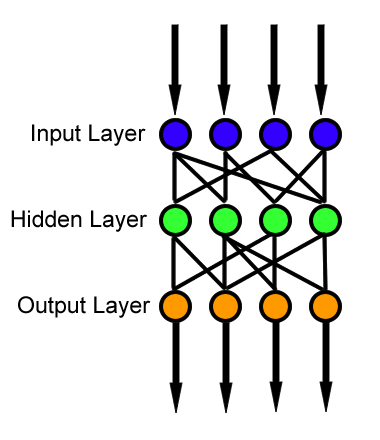
\includegraphics[width=2.5in]{feed_forward_neural_net}
%\captio{Feed forward network}
%\label{feed_forward}
%\end{figure}

\section {Conclusion}
\label{conclusion}

\section{Future Step for this work}
Given the good results we sustained using this work using Neural Network, a good next step to put this work into use would be to fit this 
trained neural network into a mobile device. Considerations must be paid to creating an efficient implementation for the network so that 
it doesn't drain the mobile device's battery.
% Generate the bibliography.
\bibliography{report}{}
\bibliographystyle{plain}
\end{document}
